\documentclass[a4paper]{article}
\usepackage{listings}
\usepackage{qtree}
\usepackage{xcolor}
\usepackage{forest}
\usepackage{multicol}
\setlength{\columnsep}{3cm}
\usepackage{parskip}
\usepackage{changepage}
\usepackage[T1]{fontenc}
\usepackage{amsmath}
\usepackage{hyperref}
\usepackage{listings}
\usepackage{amsthm}
\usepackage{amssymb}
\usepackage{float}
\usepackage[utf8]{inputenc}
\usepackage{graphicx}
\usepackage[italian]{babel}
\usepackage{thmtools}
\graphicspath{{figures/}}

\begin{document}

\author{Lorenzo Dentis, lorenzo.dentis@edu.unito.it}
\title{Esercizio finale}
\maketitle

\subsection{Introduzione}
L’esercizio consiste nella verifica di 3 proprietà in diverse varianti di un algoritmo di mutua esclusione presentato sul libro a partire dall’algoritmo 3.2 fino all’algoritmo 3.10 denominato Algoritmo di Dekker.
Le 3 proprietà da verificare sono:
\begin{itemize}
	\item \textbf{Assenza di deadlock}: Se qualche processo cerca di accedere alla regione critica eventualmente un processo potrà farlo.
	\item \textbf{Mutua esclusione}:  le istruzioni delle sezioni critiche di due o più processi non possono essere eseguite in modo interfogliato.
	\item \textbf{Assenza di starvation individuale}: Se un processo cerca di accedere alla regione critica eventualmente quel processo potra' farlo.
\end{itemize}

\section{Algoritmo 3.2}
\label{SEC:3.2}
\begin{center}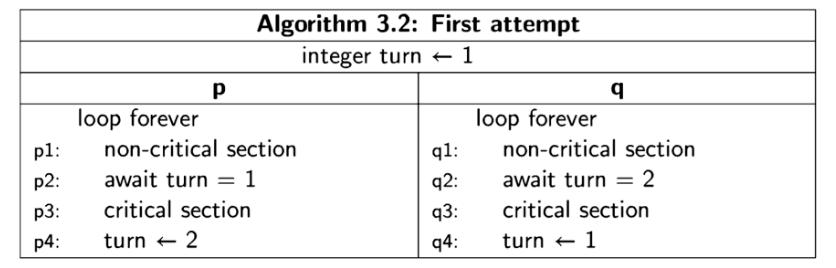
\includegraphics[width=1\textwidth]{3.2.png}\end{center}
Questo primo algoritmo propone la mutua esclusione tramite una singola variabile \textit{turn} che identifica quale processo tra \textit{p} e \textit{q} può accedere alla regione critica.
Questo algoritmo rispetta i criteri di \textbf{Assenza di deadlock \textbf{e} Mutua esclusione} ma non garantisce l' \textbf{Assenza di starvation individuale}
\newpage
\subsection{Rete di Petri}
\begin{figure*}[!ht]
\centering
\makebox[\textwidth][c]{
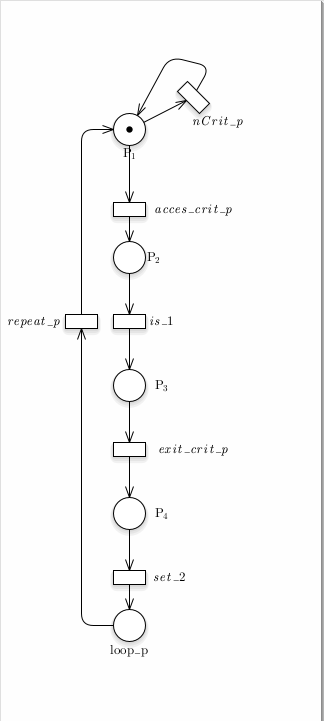
\includegraphics[width=0.5\textwidth]{p3.2.png}
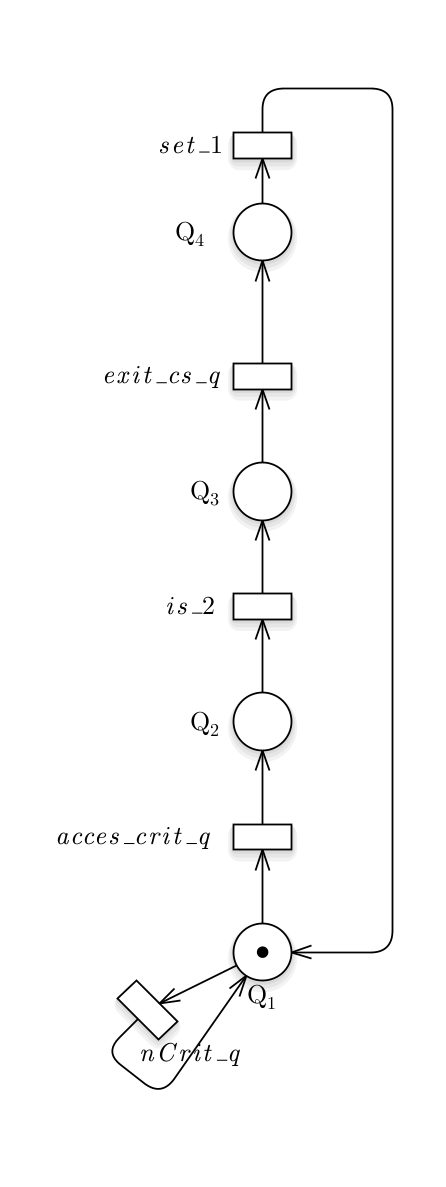
\includegraphics[width=0.5\textwidth]{q3.2.png}
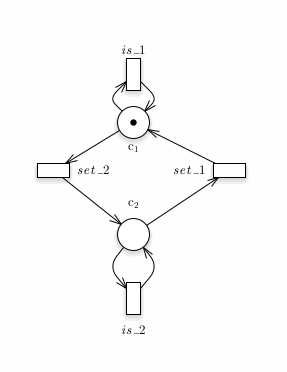
\includegraphics[width=0.5\textwidth]{variable3.2.png}}
\caption{Rete di petri decomposta} \label{FIG:decomposed3.2PN}
\end{figure*}
\begin{figure*}[!ht]
\centering
\makebox[\textwidth][c]{
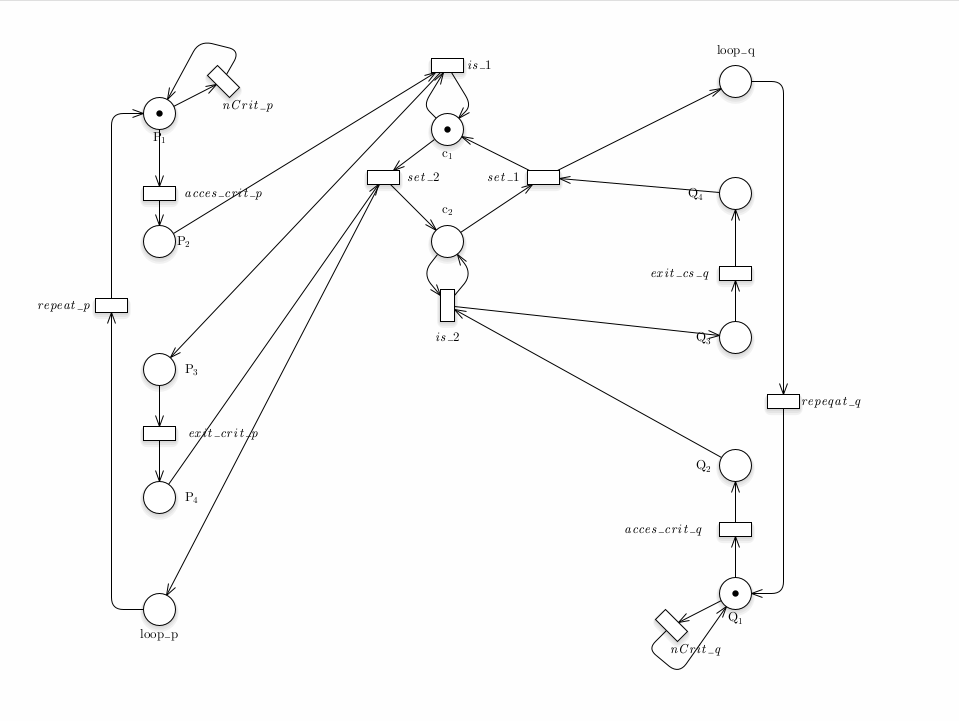
\includegraphics[width=1\textwidth]{3.2PN.png}}
\caption{Rete di petri composta} \label{FIG:3.2PN}
\subsubsection{Analisi strutturale}
\subsubsection{model checking}
\end{figure*}

\end{document}
